\documentclass[numbering=fraction]{beamer}

\usepackage[utf8]{inputenc}
\usepackage[T1]{fontenc}
\usepackage[french]{babel}
\usepackage{blindtext}
\usepackage{tikzsymbols}
\usepackage{graphicx}
\usepackage{wrapfig}
\usepackage{bookman}
\usepackage{subcaption}
\usepackage[export]{adjustbox}



\usetheme[progressbar=frametitle]{metropolis}

%Define colors
\definecolor{wuppergreen}{RGB}{85, 171, 38}
\definecolor{background}{RGB}{255,255,255}

%Adding logo to title page
\titlegraphic{\raggedleft 
\includegraphics[width=3cm]{UNamur.png}}

%Adjust color theme
\setbeamercolor{frametitle}{bg=wuppergreen}
\setbeamercolor{title separator}{fg=wuppergreen}
\setbeamercolor{footline}{fg=gray}
\setbeamercolor{progress bar}{fg=black}

%Adding footer
\setbeamertemplate{frame footer}{\insertshortauthor~(\insertshortinstitute)}

\graphicspath{ {../Images/}}

%Set parameters for title page
\title{PIMS : Sprint Review 4}
\author[PIMS]{Luis Dierick \and Gaillard Matthys \and Bouncer Yassine \and Fundu Oliver \and Anderson Rosny \and Tom Marchal }
\institute{Université de Namur}
\date{\today}

\begin{document}

\begin{frame}[plain]{}
    \maketitle
\end{frame}

\begin{frame}{Table des matières}
    \tableofcontents
\end{frame}
\section{Rappel des événements de ce qu'il y a été fait}
\begin{frame}{Rappel}
    \begin{itemize}
        \item \textbf{Sprint 1} :
        \begin{itemize}
            \item Enquête de terrain : cellule TICE 
            \item Enquête de terrain : professeurs : Englebert Vincent, Vice-doyenne
            \item Inspection des différentes technologies : \textit{django, sprint}
        \end{itemize}
        \item \textbf{Sprint 2} : 
        \begin{itemize}
            \item Écriture de mockups
            \item Écriture de scénarios
            \item Écriture de lexique, glossaire
            \item Inspection des différents utilisateurs
        \end{itemize}
        \item \textbf{Sprint 3} :
        \begin{itemize}
            \item Création de la base de données : les différents schémas
            \item Continuation de l'écriture de scénarios
            \item Première ébauche de l'interface graphique, page d'accueil, connexion, cartes des cours, création des sujets
        \end{itemize}
    \end{itemize}
\end{frame}
\subsection{Ce qui a été fait durant ce sprint}
\begin{frame}{Burndown chart}
    \centering
    
    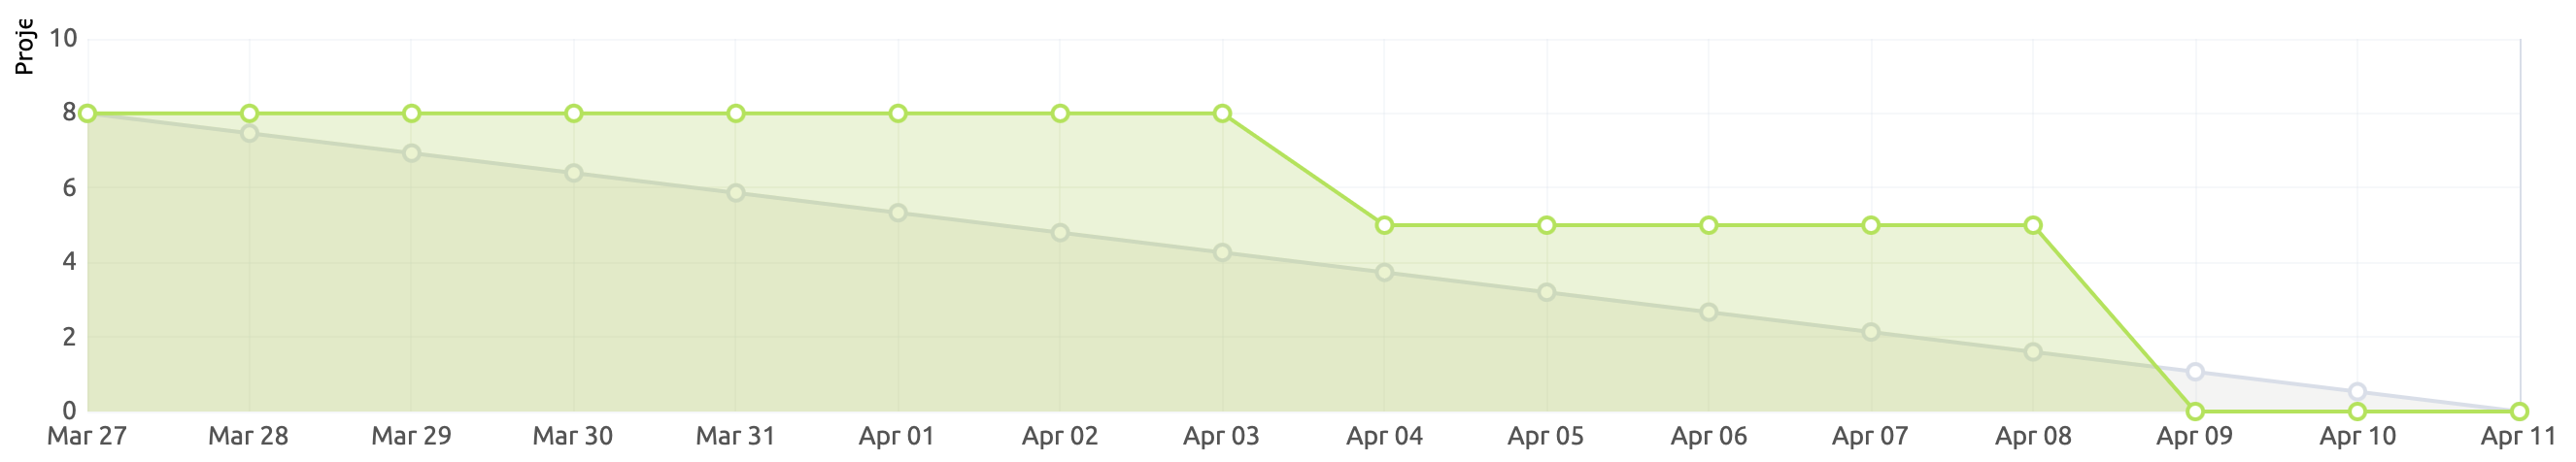
\includegraphics[width=1.1\textwidth]{burndownChart.png} 
\end{frame}

\subsection{Partie administration}
\begin{frame}{Partie administration}
    \begin{enumerate}
        \item Création de la partie administration
        \item Gestion des rôles
        \item Changements de rôles ?
    \end{enumerate}
\end{frame}
\subsection{Inscription à un cours}
\begin{frame}{Inscription à un cours et visualisation d'un cours}
    \begin{enumerate}
        \item 2 parties
        \begin{itemize}
            \item Inscription
            \item Affichage des cours auquel on est inscrit.
        \end{itemize}
    \end{enumerate}
\end{frame}
\subsection{Modification d'un sujet}
\begin{frame}{Modification d'un sujet}

    \begin{enumerate}
        \item Modification d'un sujet
        \item Suppression d'un sujet
    \end{enumerate}
\end{frame}
\section{Scénarios}
\begin{frame}{Scénarios}
    \begin{itemize}
        \item Correction du scénario de l'admin (FIGMA).
        \item Correction de l'écriture des scénarios.
    \end{itemize}
\end{frame}
\section{Echéances prévues}
\begin{frame}{Echéances prévues}
    \begin{enumerate}
        \item Terminer le plus possibles selon l'ordre des priorités les pages web.
        \item Terminer les scénarios d'utilisation
        \item Planification de la prochaine réunion.
    \end{enumerate}
\end{frame}

\end{document}